\documentclass{assignment}
\usepackage[utf8]{inputenc}
\usepackage[T1]{fontenc}
\usepackage{hyperref}
\usepackage{listings}

%\lstset{
%	inputencoding=utf8,
%	literate=
%	{á}{{\'a}}1
%	{é}{{\'e}}1
%	{í}{{\'i}}1
%	{ó}{{\'o}}1
%	{ú}{{\'u}}1
%	{Á}{{\'A}}1
%	{É}{{\'E}}1
%	{Í}{{\'I}}1
%	{Ó}{{\'O}}1
%	{Ú}{{\'U}}1
%	{ñ}{{\~n}}1
%	{Ñ}{{\~N}}1
%}
%
%
%\lstdefinelanguage{Pseudocodigo}{
%	morekeywords={
%		SI, ENTONCES, SINO, FIN, MIENTRAS, HACER, PARA, DESDE, HASTA,
%		FUNCIÓN, PROCEDIMIENTO, CLASE, CONSTRUCTOR, ATRIBUTOS,
%		RETORNAR, ALGORITMO, CONSTANTE, NUEVO, Y, O, NO, CADA, EN
%	},
%	sensitive=false,
%	morecomment=[l]{//},
%	morestring=[b]",
%}
%
%\lstset{
%	language=Pseudocodigo,
%	basicstyle=\ttfamily\small,
%	keywordstyle=\color{blue}\bfseries,
%	commentstyle=\color{gray}\itshape,
%	stringstyle=\color{orange},
%	numbers=left,
%	numberstyle=\tiny\color{gray},
%	stepnumber=1,
%	breaklines=true,
%	frame=single,
%	tabsize=4,
%	showstringspaces=false,
%}
\begin{document}
	
	\assignmentTitle{Claudio Iván Esparza Castañeda}{Luis Alberto Balam Guzmán}{./Logo.png}{Maestría en Sistemas Embebidos}{Programación y Procesamiento de Datos}{4A. Práctica de tratamiento de señales en sistemas embebidos con Python}
	\section*{Objetivo}
	Lo que hizo Arduino por la cultura maker fue fundamental para democratizar la tecnología. Por otro lado, otro impulso se dio a través del uso de Python por la misma comunidad (junto a su creador, Guido Van Rossum). En algún punto estas dos fuerzas convergieron para llegar a micropython, que es un proyecto que empuja hacia esta democratización para el tipo de usuario que en su día a día no tiene tiempo de aprender todo acerca del hardware, pero busca realizar proyectos de fin de semana, o bien el profesional o el estudiante que requiere un prototipado rápido para el proyecto de fin de semana. Después del Arduino, han aparecido diferentes soluciones con distintos controladores. Así es como llegamos a la Raspberry Pi Pico, que se puede programar a través de bare-metal, con RTOS (FreeRTOS, Zephyr, etc.), o micropython.\\
	Con la imposibilidad que representa tener que procesar grandes cantidades de información en un medio con pocos recursos, refiriéndonos en este caso a la Raspberry Pi Pico, surge la necesidad de contar con sistemas híbridos: control en el sistema embebido, y procesamiento en la computadora.
	\section*{Descipción de la solución}
	Se sigue la estructura propuesta para el proyecto. Hay un único cambio realizado en el archivo {\tt generador\_senial.py} fue renombrarlo a {\tt main.py} e incluirlo en la carpeta {\tt pico}$\slash$, Este cambio se realizó con el objetivo de poder usar el puerto serial sin que se bloqueé el puerto serial por el REPL.\\
	Por otro lado, se dividieron responsabilidades a través de las distintas partes requeridas. Por un lado, el archivo {\tt captura.py} se autodescribe. Se encarga de establecer la conexión del puerto y recibir la información procedente de la tarjeta. El archivo {\tt procesamiento.py} también se autodescribe, contiene las operaciones científicas de los módulos de Python, de acuerdo a lo requerido. El archivo {\tt visualizacion.py} contiene las funciones encargadas de la creación de las gráficas.\\
	Se sigue usando el archivo {\tt funciones.py} de tareas anteriores, con el objetivo de hacer algunas validaciones. El archivo {\tt main.py} se encarga de ejecutar todo lo anterior en el orden dado.
	\section*{Metodología}
	El tratamiento de las señales se realiza con SciPy, al emplear las funciones definidas en este módulo. Primeramente se encuentra un filtro pasa-bajas tipo Butterworth de 4 orden. Se comprobó que no hay mucha diferencia entre el filtro de segundo orden, tercero ni quinto. entre mayor sea el número de muestras conviene un filtro de mayor orden, pero para 1000 no hay una diferencia apreciable.\\
	Para la detección de picos primero se calcula la desviación estándar de la señal filtrada, y se emplea la función find\_peaks incluida en SciPy\\
	Para la detección de anomalías se calcula el residuo como la diferencia entre la señal original y la señal filtrada. Después se encuentra la desviación estándar y se obtiene los que están fuera del residuo en el orden de la desviación estándar.\\
	Por último, el análisis FFT utiliza las funciones {\tt rfft} y {\tt rfftreq} para obtener las magnitudes y frecuencias de manera casi directa.\\
	La visualización, por su parte, sólo es emplear las salidas del procesamiento para establecer los ejes de las gráficas.
	\section*{Capturas de ejecución}
	\begin{figure}[htbp]
		\centering
		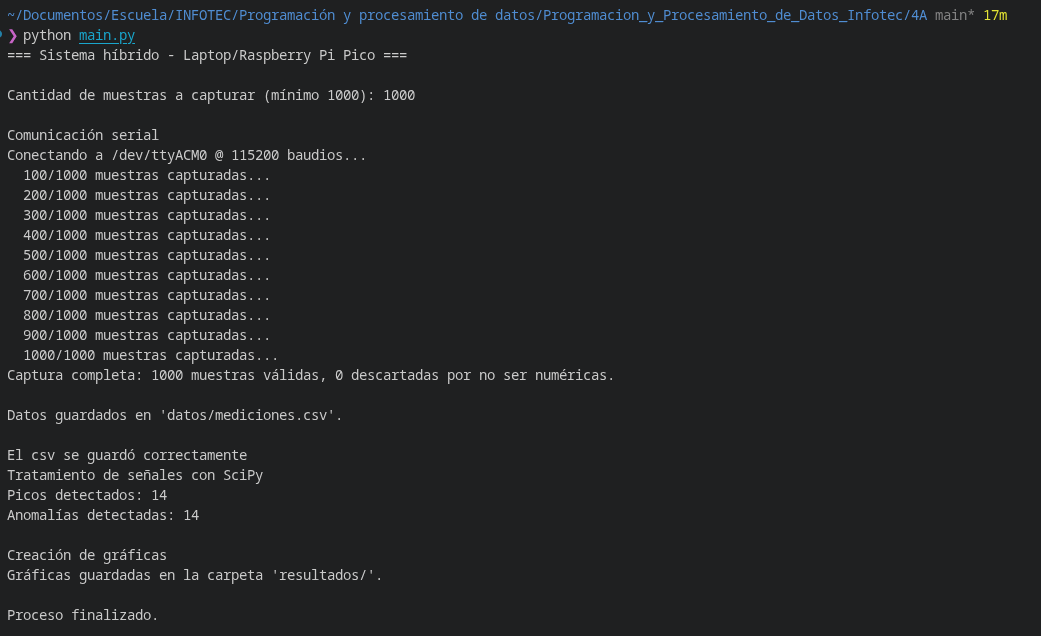
\includegraphics[width=0.8\textwidth]{Figuras/1}
		\caption{Ejecución del programa. Se pide de entrada el número de muestras a capturar..}
		\label{fig:1}
	\end{figure}
	\begin{figure}[htbp]
		\centering
		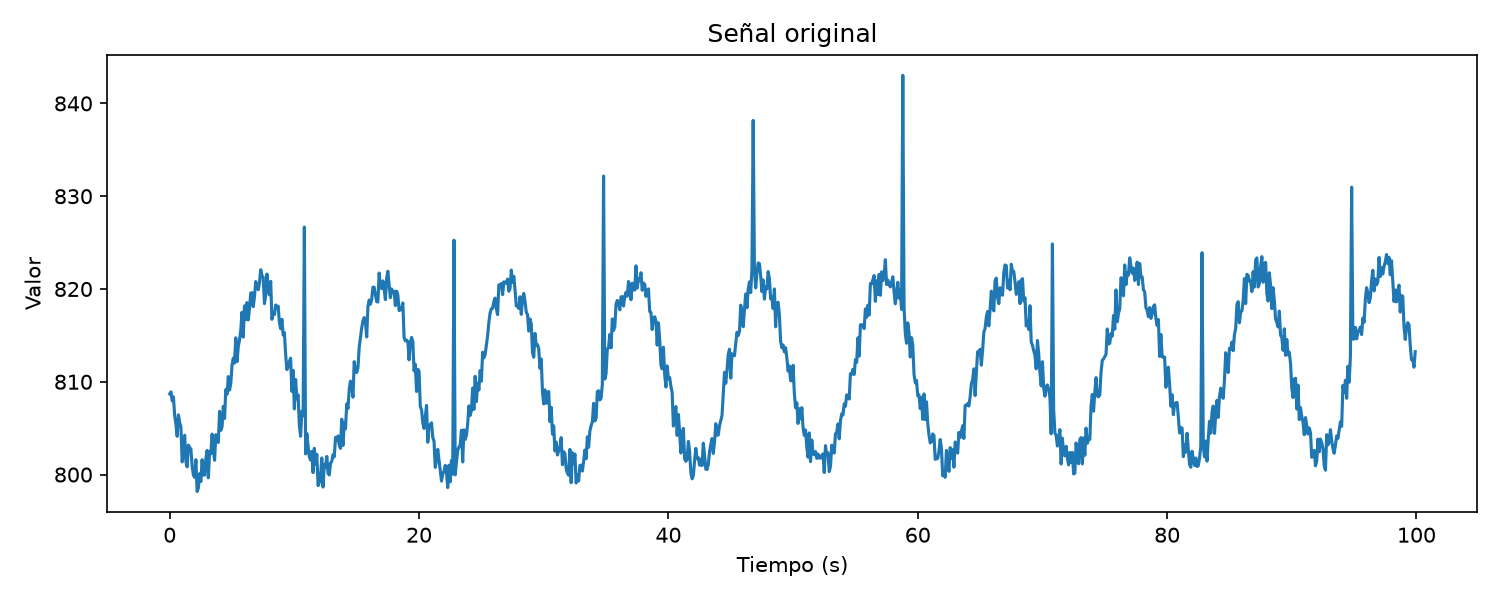
\includegraphics[width=\textwidth]{Figuras/2}
		\caption{Señal original.}
		\label{fig:2}
	\end{figure}
	\begin{figure}[htbp]
		\centering
		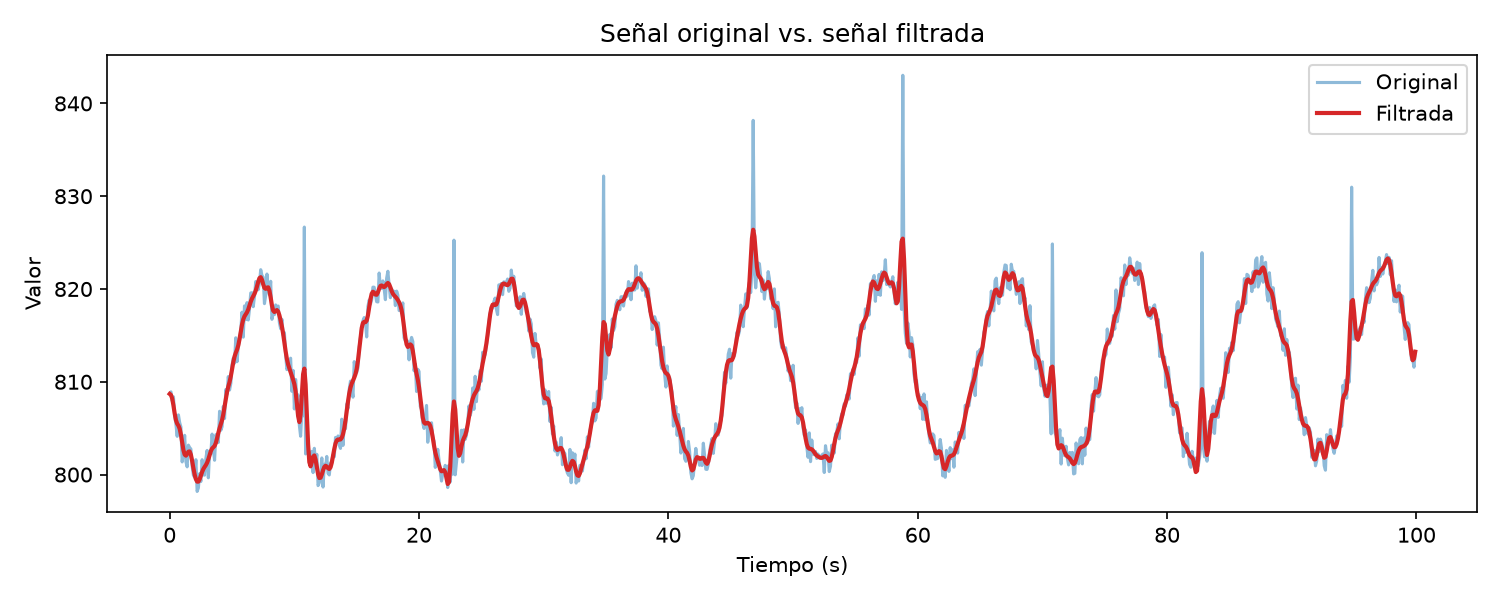
\includegraphics[width=\textwidth]{Figuras/3}
		\caption{Señal original vs. señal filtrada}
		\label{fig:3}
	\end{figure}
	\begin{figure}[htbp]
		\centering
		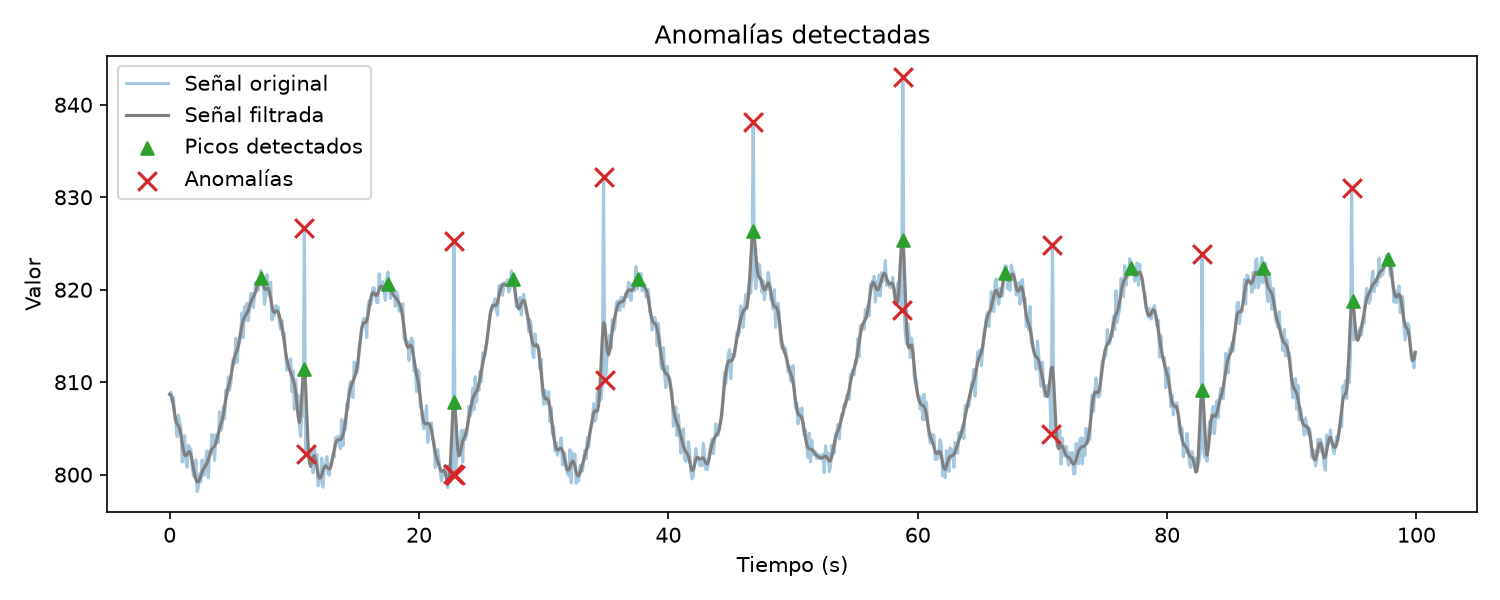
\includegraphics[width=\textwidth]{Figuras/4}
		\caption{Anomalías detectadas.}
		\label{fig:4}
	\end{figure}
	\begin{figure}[htbp]
		\centering
		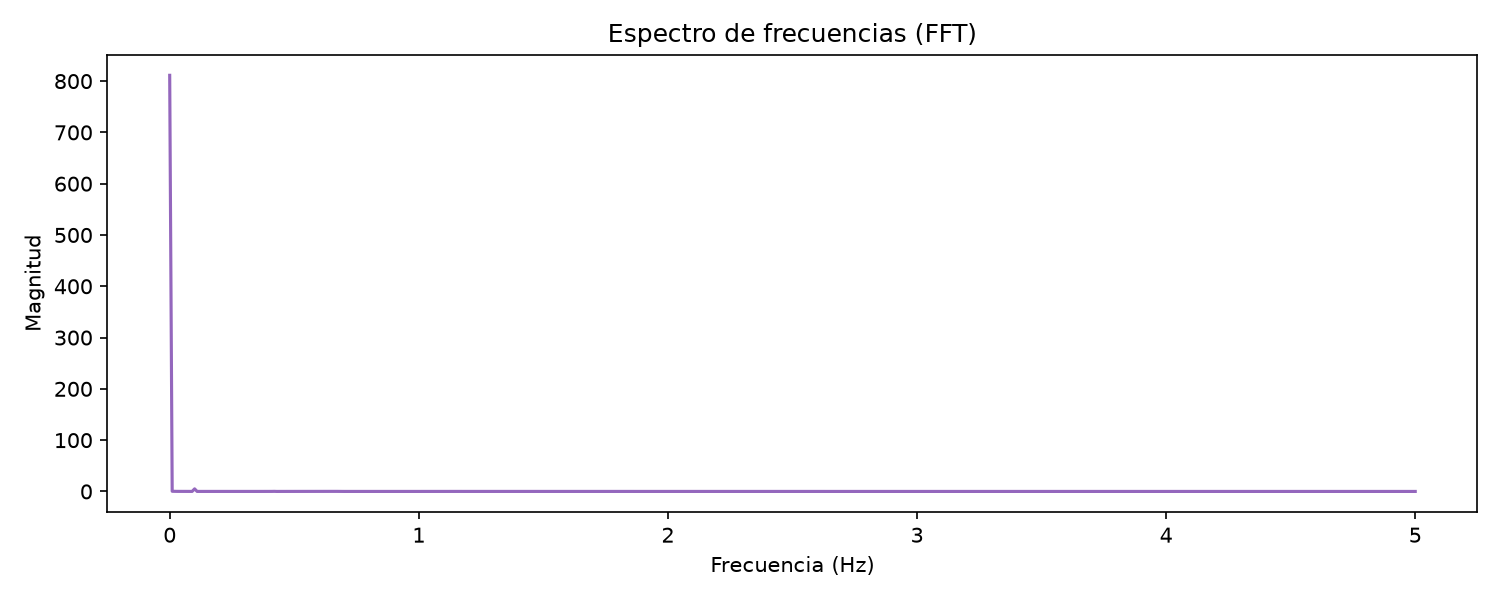
\includegraphics[width=\textwidth]{Figuras/5}
		\caption{Transformada rápida de Fourier (FFT).}
		\label{fig:5}
	\end{figure}
	\section*{Conclusiones}
	MicroPython permite crear prototipos rápidos para interactura con hardware y tomar mediciones del ambiente. Con esto permite su uso en el mundo maker, artístico e ingenieril, por mencionar algunos. Trabajar de manera híbrida permite que la placa se encargue del control y adquisición de datos, mientras que la computadora, más potente, se encargue del procesamiento.\\
	La carpeta en el repositorio de este proyecto es: \href{https://github.com/clivan/Programacion_y_Procesamiento_de_Datos_Infotec/4A}{Programación y procesamiento de Datos}.	
\end{document}
